Une large partie de la théorie des données fonctionnelles suppose que l'on observe des courbes $X_i : \Omega \rightarrow \mathcal C^0(I, \mathds R)$ \textbf{indépendantes} et identiquement distribuées. Cependant une partie non négligeable des données que l'on observe ont des dépendances avec les valeurs passées. Par exemple, il est raisonnable de penser que la consommation électrique d'un foyer au cours d'une année croît avec l'ajout successif de nouveau appareils électroniques. L'hypothèse d'indépendance entre les données n'est donc plus pertinente pour les données que l'on traite et il devient important de considérer des processus autorégressifs adaptés aux données fonctionnelles.
Si dans le cadre des données de $\mathds R$ cette relation de \emph{dépendance linéaire} avec le passé pouvait s'écrire sous la forme suivante
$X_n = \sum\limits_{k=1}^{n-1} \varphi_k \, X_k + \xi_n$ où $\varphi_k \in \grandR$
et
$\xi_n \begin{cases} \in \operatorname{VA}(\grandR) \\ \indep \sigma\left( X_i \right)_{1\,: \, n-1}\end{cases}$,
dans le cadre fonctionnel on capture la même idée en considérant
$X_n = \sum\limits_{k=1}^{n-1} \phi_k \left( X_k \right) + \xi_n$ où $\phi_k$
est un \emph{opérateur linéaire} de $\mathds L^2(I, \mathds R)$,
le plus souvent intégral.

\chk{
	Il s'agit d'une généralisation naturelle de la relation dans le cadre réel, puisqu'on peut démontrer que sur l'espace des nombres réels l'ensemble des fonctions linéaires $\phi : \grandR \rightarrow \grandR$ sont de la forme $x \mapsto ax$ avec $a \in \grandR$. La relation sur $\grandR$ que l'on a vue juste avant peut alors se ré-écrire de façon similaire à la version fonctionnelle.
}

On considère lors de ce stage des séries temporelles de données fonctionnelles car les données que l'on manipule ( en l'occurence les données de courbe de charge des parcs éoliens ) semblent être naturellement corrélées dans le temps.


\question{Pourquoi se soucier en particulier des séries temporelles fonctionnelles lorsque l'on souhaite incorporer la régularité du processus dont est issu nos données dans l'estimation des quantités qui nous intéressent ?}

Rappelons-nous que les données fonctionnelles sont la clé pour déterminer la régularité, et que cela est en réalité permis par le théorème de \nameref{rem:kolmo_continuite} (que nous n'avons pas énoncé en détails, mais mentionné dans la section \ref{sec:informel}). Malheureusement, dans le monde réel où vit le praticien, nous n'avons pas accès à l'espérance de la loi dont sont issues nos données. Il nous faut donc estimer cette espérance, et c'est là que les séries temporelles fonctionnelles entrent en jeu. Puisque l'estimateur usuel de l'espérance est la moyenne empirique, qui nous est fourni par la loi des grands nombres, cela devient très problématiques lorsque l'on dispose de données corrélées.
% TODO ✏️ mieux formuler - dépendance faible -> LGN faible -> estim esperance
Ce que nous allons voir, c'est que l'on peut tout de même utiliser l'estimateur usuel de l'espérance, et que l'on obtiendra des estimateurs des paramètres de régularité convergents ponctuellement vers ceux du processus dont sont issues nos données. Ce résultat est dérivé en utilisant une forme particulière de dépendance que le lecteur pourra étudier plus en détail en annexe \ref{annexe:regularite-locale}.

\begin{figure}[H]
	\centering
	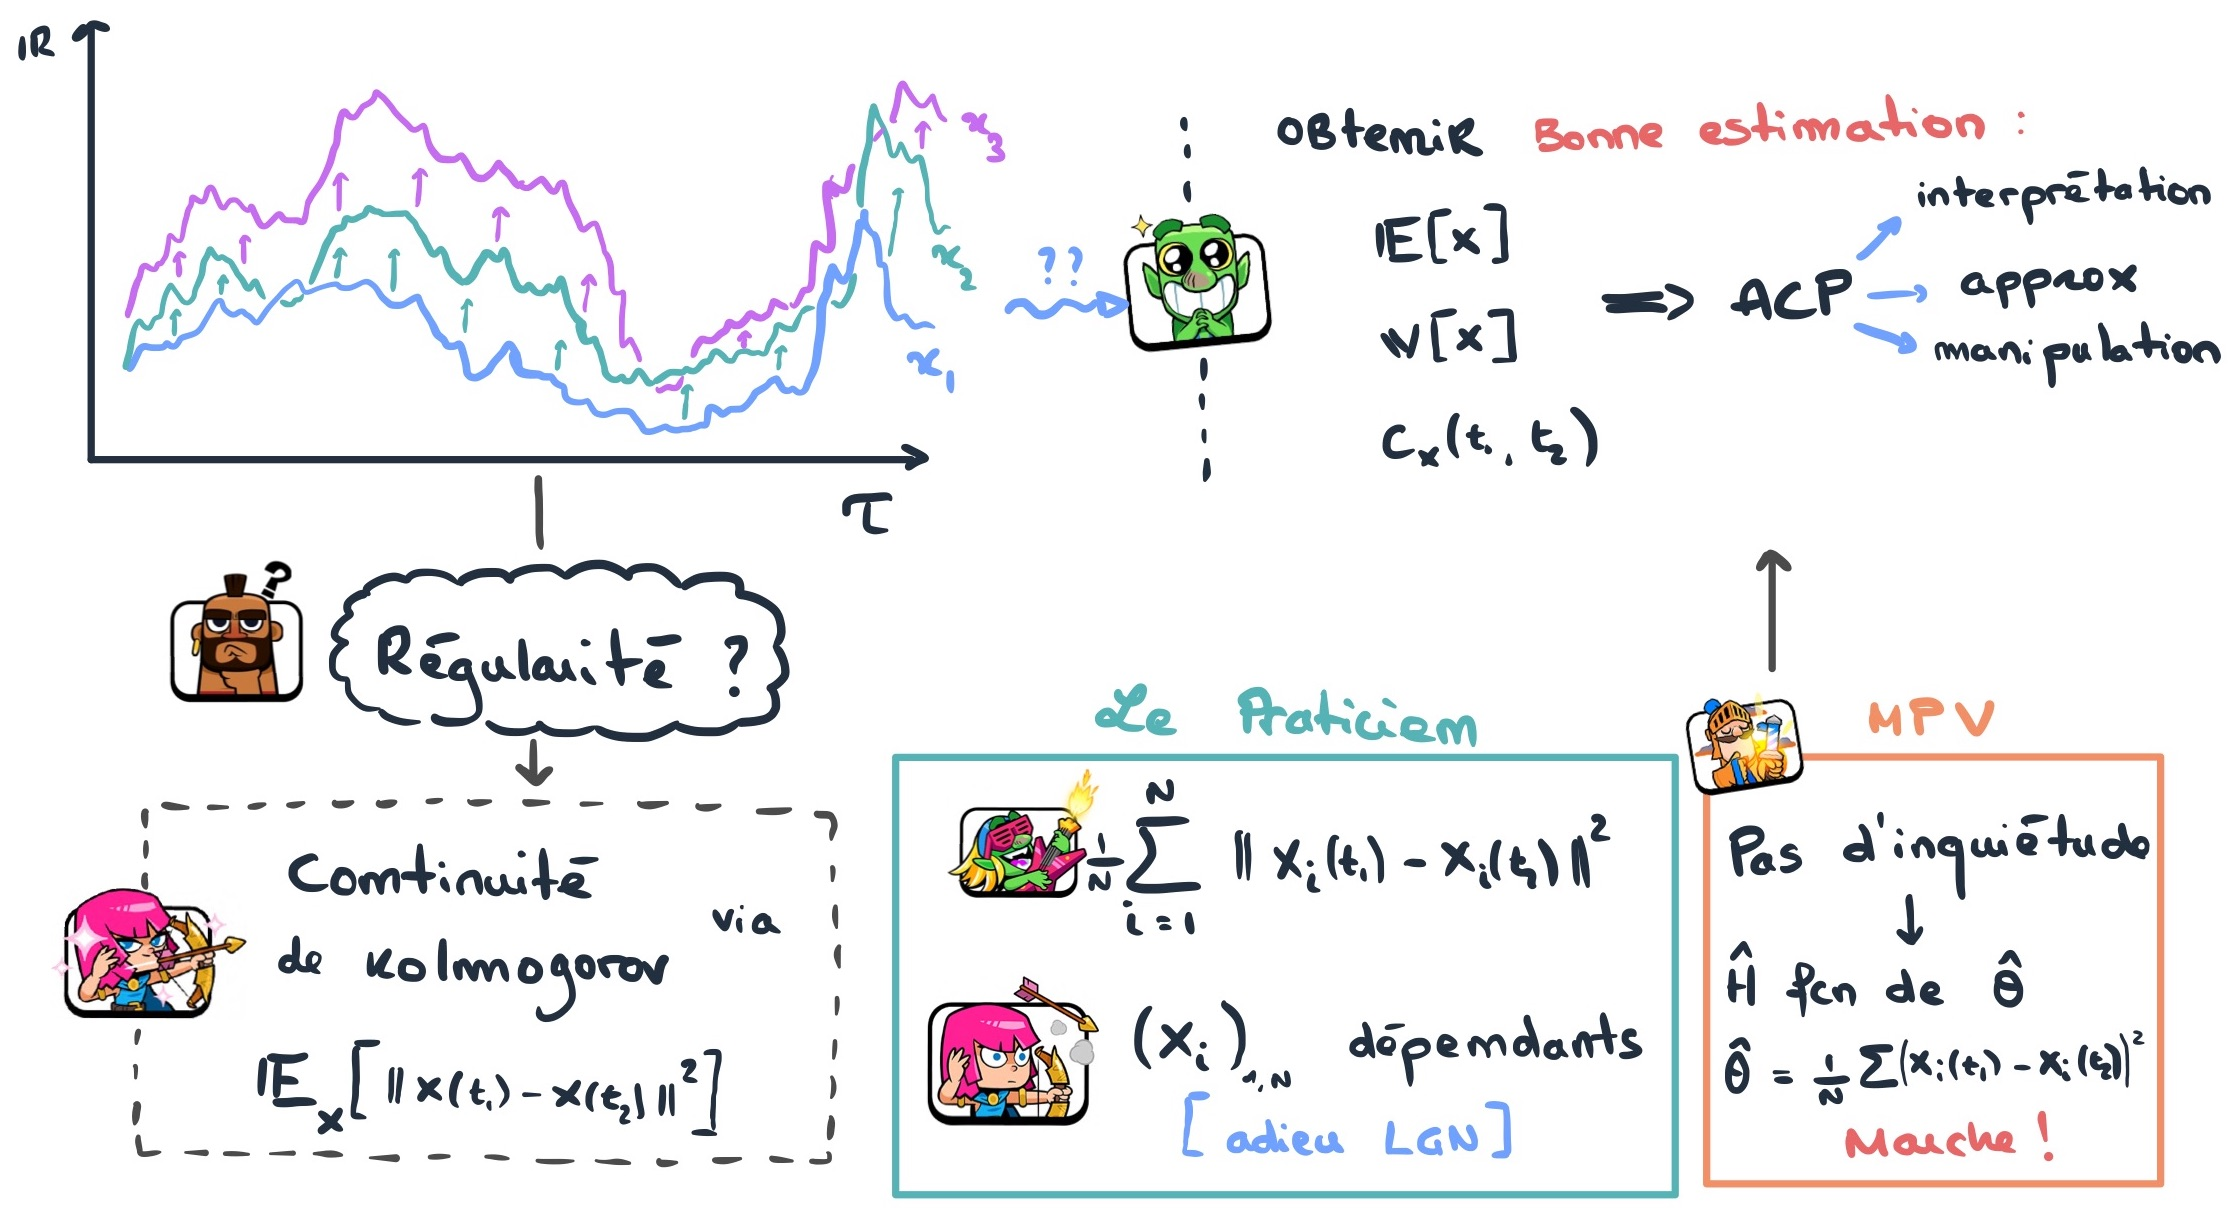
\includegraphics[width=\textwidth]{Images/sketches/schema_ts_estim_reg.jpg}
	\caption{Schéma grossièrement récapitulatif : Estimation de la régularité pour une série temporelle fonctionnelle}
	\label{fig:recap_estim_reg_fts}
\end{figure}


\warn{Il faut faire attention lorsque l'on manipule ou interprète des séries temporelles fonctionnelles. (comme par exemple tout résultat utilisant la loi de $\sum\limits_n X_n$, ... )}

Une série temporelle discrète est le fait que l'observation suivante dépend linéairement de l'observation précédente, dans le cadre fonctionnel \emph{l'observation est une fonction}. La dépendance se fait sur l'indice de la fonction, et non pas sur l'argument de la fonction interprété dans notre caps comme étant le temps.

\bigskip

Dans le cadre éolien c'est d'autant plus trompeur de parler de temps car on observe des courbes de charge sur une année : à la fois l'indice de la fonction et l'argument de la fonction ont des interprétations temporelles.

\smallskip

\noindent\fbox{%
    \parbox{\textwidth}
    {%
        dans l'expression \og$X_n(t)$\fg, la série temporelle (discrète) concerne bien l'indice $n$ et non pas l'argument $t$.
    }
}

\bigskip

\noindent La question devient alors :
\question{Lorsque l'on a une dépendance dans les observations fonctionnelle $\left\{ X_1 \dots X_n \right\}$, possède-t-on une dépendance dans les observations ponctuelles à $t$ fixé $\left\{ X_1(t) \dots X_n(t) \right\}$ ? Cette dépendance est-elle la même ?}

\noindent Et la réponse, c'est qu'\textbf{on ne sait pas}. En tout cas, dans le cadre général. Il y a en effet plusieurs façon de définir ce qu'on appelle par \og dépendance temporelle \fg. Toutes les définitions de dépendance ne mènent pas à cette conclusion, mais celle adoptée par (MPV) l'est, étant plus faible. De manière générale, lorsque l'on traîte des données avec de la dépendance, il convient d'être extrêmement précautionneux avec les théorèmes et \og faits \fg que l'on invoque. Toujours bien vérifier les hypothèses.

\bigskip
\noindent\fbox{\parbox{\textwidth}{%
		\noindent La dépendance faible comme définie dans l'article de MPV\cite{maissoro-SmoothnessFTSweakDep} nous permet de travailler localement : On peut travailler localement sur les trajectoires tout en utilisant des hypothèses fonctionnelles (que ce soit pour la dépendance ou autres) pour obtenir la régularité.}}

\input{content/chapter_2/01-fda_essentiel/03-time_series/01-03-simulation.tex}